\documentclass[letterpaper]{article}
\usepackage[margin=1in]{geometry}
\usepackage[utf8]{inputenc}
\usepackage{textcomp}
\usepackage{amssymb}
\usepackage{natbib}
\usepackage{graphicx}
\usepackage{gensymb}
\usepackage{amsthm, amsmath, mathtools}
\usepackage[dvipsnames]{xcolor}
\usepackage{enumerate}
\usepackage{mdframed}
\usepackage[most]{tcolorbox}
\usepackage{csquotes}
% https://tex.stackexchange.com/questions/13506/how-to-continue-the-framed-text-box-on-multiple-pages

\tcbuselibrary{theorems}

\newcommand{\R}{\mathbb{R}}
\newcommand{\Z}{\mathbb{Z}}
\newcommand{\N}{\mathbb{N}}
\newcommand{\Q}{\mathbb{Q}}
\newcommand{\C}{\mathbb{C}}
\newcommand{\code}[1]{\texttt{#1}}
\newcommand{\mdiamond}{$\diamondsuit$}
\newcommand{\PowerSet}{\mathcal{P}}
\newcommand{\Mod}[1]{\ (\mathrm{mod}\ #1)}
\DeclareMathOperator{\lcm}{lcm}

%\newtheorem*{theorem}{Theorem}
%\newtheorem*{definition}{Definition}
%\newtheorem*{corollary}{Corollary}
%\newtheorem*{lemma}{Lemma}
\newtheorem*{proposition}{Proposition}


\newtcbtheorem[number within=section]{theorem}{Theorem}
{colback=green!5,colframe=green!35!black,fonttitle=\bfseries}{th}

\newtcbtheorem[number within=section]{definition}{Definition}
{colback=blue!5,colframe=blue!35!black,fonttitle=\bfseries}{def}

\newtcbtheorem[number within=section]{corollary}{Corollary}
{colback=yellow!5,colframe=yellow!35!black,fonttitle=\bfseries}{cor}

\newtcbtheorem[number within=section]{lemma}{Lemma}
{colback=red!5,colframe=red!35!black,fonttitle=\bfseries}{lem}

\newtcbtheorem[number within=section]{example}{Example}
{colback=white!5,colframe=white!35!black,fonttitle=\bfseries}{def}

\newtcbtheorem[number within=section]{note}{Important Note}{
        enhanced,
        sharp corners,
        attach boxed title to top left={
            xshift=-1mm,
            yshift=-5mm,
            yshifttext=-1mm
        },
        top=1.5em,
        colback=white,
        colframe=black,
        fonttitle=\bfseries,
        boxed title style={
            sharp corners,
            size=small,
            colback=red!75!black,
            colframe=red!75!black,
        } 
    }{impnote}
\usepackage[utf8]{inputenc}
\usepackage[english]{babel}
\usepackage{fancyhdr}
\usepackage[hidelinks]{hyperref}

\pagestyle{fancy}
\fancyhf{}
\rhead{Math 170B}
\chead{Monday, June 05, 2023}
\lhead{Lecture 27}
\rfoot{\thepage}

\setlength{\parindent}{0pt}

\begin{document}

\section{Genetic Algorithms and Convex Programming (Section 11.7)}
This section will go over both generic algorithms and convex programming. 

\subsection{Genetic Algorithms}
Inspired by observations in the biological sciences, \textbf{generic algorithms} can be used to solve combinatorial and discrete problems. Let's suppose we have a function $f(x)$. We don't know the minimum value of $f(x)$, only that its minimum value is greater than or equal to 0. In other words, $f(x) \geq 0$.

\bigskip 

Suppose we have a population of $x^{(1)}, x^{(2)}, \hdots$, which are solution estimates. We want to use $\frac{1}{F(x^{(i)})}$ as proxies for probabilities. Picking the solution estimates with high probabilities, we can recombine that solution estimates to form a new ``generation'' of solution estimates. 


\subsection{Convex Sets and Functions}
We say that $f$ is convex if it is defined on a convex set $K$ and satisfies a condition. Before we go over the condition, let us define what a convex set is.
\begin{definition}{Convex Set}{}
    A \textbf{convex set} is a set $K$ such that, for $x, y \in K$ and $0 \leq \theta \leq 1$, 
    \[\theta x + (1 - \theta) y \in K.\]
\end{definition}
In other words, for any two points in the set, the set contains the line between the two points.
\begin{center}
    \begin{tabular}{p{3in}| p{3in}}
        \textbf{Convex Set} & \textbf{Not Convex Set} \\ 
        \hline 
        \begin{center}
            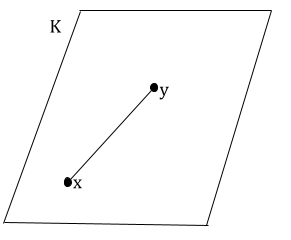
\includegraphics[scale=0.5]{../assets/convex_set.png}
        \end{center}
        & 
        \begin{center}
            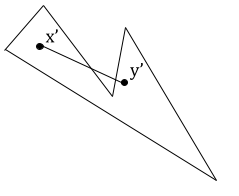
\includegraphics[scale=0.5]{../assets/not_convex_set.png}
        \end{center}
    \end{tabular}
\end{center} 

With this in mind, a convex function is analogous to a convex set; consider the visualization below:
\begin{center}
    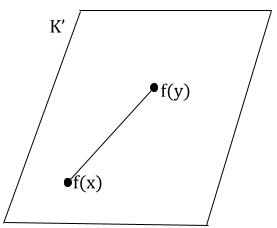
\includegraphics[scale=0.5]{../assets/convex_funcset.png}
\end{center}
But, we're considering the function values instead. So, if $f(x)$ and $f(y)$ form a line and that line remains within the set of function values, then that function is convex. More formally, for $x, y \in K'$ and $0 \leq \alpha \leq 1$, we have \[\alpha f(x) + (1 - \alpha) f(y) \in K'.\]

\subsection{Linear Inequalities \& Consistent Systems}
Fix $x \in \R^n$. Each linear inequality is defined by the constant $a_{ji}x_{i} - b_{j} \geq 0$. This, in turn, means that 
\[\sum_{i = 1}^{n} a_{ji}x_{i} - b_{j} \geq 0 \qquad i \leq j \leq m.\]
This corresponds to the matrix inequality,
\[Ax - b \geq 0.\]
How do we know if the system is \emph{consistent}? We say that a system is consistent if it has at least \emph{one} solution.
\begin{mdframed}
    (Example.) Suppose $m = 3$ and $n = 2$, and suppose we have the system
    \[\begin{bmatrix}
        1 & 1 \\ 
        1 & -1 \\ 
        -3 & 1
    \end{bmatrix} \begin{bmatrix}
        x_1 \\ x_2
    \end{bmatrix} - \begin{bmatrix}
        2 \\ -1 \\ -6
    \end{bmatrix} \geq \begin{bmatrix}
        0 \\ 0 \\ 0 
    \end{bmatrix}.\]
    The corresponding inequalities are:
    \begin{equation*}
        \begin{aligned}
            x_1 + x_2 &\geq 2 \\ 
            x_1 - x_2 &\geq -1 \\ 
            -3x_1 + x_2 &\geq -6.
        \end{aligned}
    \end{equation*}
    In the two-dimensional case, we can plot the system and see what the corresponding regions are. By rewriting the system as appropriate, the resulting plots are shown below: 
    \begin{center}
        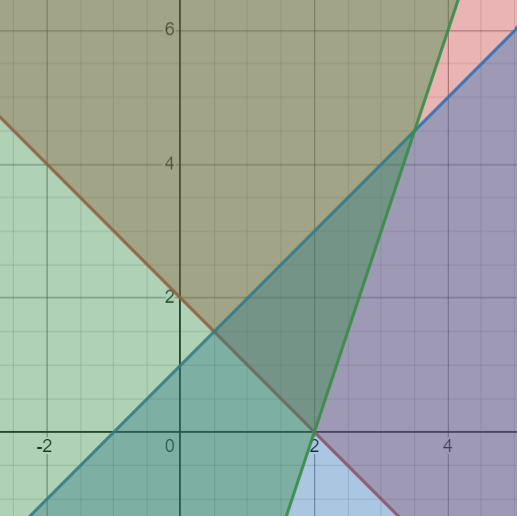
\includegraphics[scale=0.7]{../assets/consistent1.png}
    \end{center}
    The feasible region is defined by the intersection of all three inequalities. In this case, the triangle where the three inequalities overlap above is our feasible region. This also defines our convex set: if we choose any two points in that region, and any linear combination, then the resulting line will remain in this region. 
\end{mdframed}
So, to summarize:
\begin{itemize}
    \item The feasible region is defined by the intersection of all constraints (e.g., inequalities). 
    \item If the feasible region is \emph{empty}, then the system is inconsistent.
\end{itemize}

\subsection{Convex Programming}
In this area, a convex function can be approximated by 
\[F(x) = \max_{1 \leq i \leq j} \left(\sum_{j = 1}^{n} a_{ij} x_j - b_i\right).\]
The convex domain is approximated by the set \[K = \{x : G(x) \leq 0\},\] where \[G(x) = \max_{k < i \leq m} \left(\sum_{j = 1}^{n} a_{ij}x_j - b_i\right).\]
One way to condense this is to represent this problem in terms of a matrix $A$ and a vector $b$. So, we can let $A \in \R^{m \times n}$ and vector $b \in \R^m$ describe the problem. Let's suppose that each set of $n$ rows from $A$ is linearly independent\footnote{This is known as the ``Haar'' condition.}. Then, the residual value is defined by \[r_{i}(x) = \sum_{j = 1}^{n} a_{ij} x_{j} - b_{i} \qquad 1 \leq i \leq m.\]
Moving to the idea of convex programming itself, we will consider an outline of an algorithm for how convex programming (optimization) works. Generally, we start with a set of indices $J \subset \{1, 2, 3, \hdots, n\}$. Then, at each step, 
\begin{enumerate}
    \item $J$ has $n + 1$ elements. 
    \item At least one element of $J$ is in $\{1, 2, \hdots, k\}$. 
    \item The origin is in the convex hull of $\{A_{\text{row } i} : i \in J\}.$
\end{enumerate}
Also, at each step, we want to compute $x \in \R^n$ and $\lambda \in \R$ such that 
\[\begin{aligned}
    r_{i}(x) = \lambda \qquad &\text{if} \qquad i \in J \qquad (i \leq k) \\ 
    r_{i}(x) = 0 \qquad &\text{if} \qquad i \in J \qquad (i > k)
\end{aligned}\]
This process gives us the solution of the linear system with $n + 1$ unknowns and $n + 1$ equations. To turn this into a rough algorithm, given $x$ and $\lambda$, we want to compute $F(x)$ and $G(x)$.
\begin{itemize}
    \item If $G(x) \leq 0$ and $F(x) = \lambda$, we can stop.
    \item If $G(x) > 0$, we can select an index $\lambda > k$ such that $r_{\lambda}(x) > 0$.
    \item If $G(x) \leq 0$ and $F(x) > \lambda$, then we can select an index $\alpha \leq k$ where $r_{\alpha}(x) > \lambda$. 
\end{itemize} 
Essentially, we want to replace $\alpha$ with an index $\beta \in J$ so that the new index set $J'$ contains the origin in the convex hull.

\end{document}